\documentclass[11pt]{article}

\usepackage[margin=1in]{geometry}
\usepackage{microtype}
\usepackage{booktabs}
\usepackage{tabularx}
\usepackage{threeparttable}
\usepackage{placeins}
\usepackage{graphicx}
\usepackage{xcolor}
\usepackage{amsmath}
\usepackage{authblk}
\usepackage{natbib}
\usepackage{hyperref}
\usepackage[nameinlink,noabbrev]{cleveref}
\usepackage{tikz}
\usetikzlibrary{arrows.meta,positioning,fit,shapes.geometric,decorations.pathmorphing}

\setcounter{topnumber}{2}
\setcounter{totalnumber}{4}
\renewcommand{\topfraction}{0.82}
\renewcommand{\textfraction}{0.12}
\renewcommand{\floatpagefraction}{0.99}

\definecolor{bluebox}{HTML}{EAF2F8}
\definecolor{greenbox}{HTML}{EAF6EE}
\definecolor{goldbox}{HTML}{FFF4D6}
\definecolor{linegray}{HTML}{65737E}
\definecolor{measureorange}{HTML}{D97706}
\definecolor{testblue}{HTML}{2563A6}
\hypersetup{
  colorlinks=true,
  linkcolor=blue!45!black,
  citecolor=green!35!black,
  urlcolor=blue!55!black,
  pdftitle={Supervised Calibration of Unsupervised Microbiome Network Scores with Partial Experimental Measurements}
}

\newcommand{\ap}{\mathrm{AUPRC}}

\title{Supervised Calibration of Unsupervised Microbiome Network Scores with Partial Experimental Measurements}
% Replace this line with the final author and affiliation block before submission.
\author{Anonymous manuscript}


\date{}

\begin{document}
\maketitle

\begin{abstract}
Microbiome network estimators produce continuous evidence for taxon pairs without using experimental interaction labels. We developed LENS, Label-Enriched Network Scores, as a partial measurement procedure for interpreting that evidence within the microbial system where predictions are needed. LENS begins with the equal mean of score percentiles from PLNNetwork, Poisson neighborhood selection, and SparCC. Measured interactions update this reference through centred ridge logistic regression, with pair abundance features entering only when supported by the labels. When either outcome class has fewer than three measured pairs, LENS retains the fixed mean score because penalty selection is unreliable. We evaluated the procedure with five held-out pair folds and nested measurement budgets. Test pairs remained fixed across budgets, so each budget differed only in the interaction labels available for training. At the 80\% budget, mean AUPRC was 0.882 in the butyrate assembly system, 0.282 in Carlstr\"om, and 0.429 in Sch\"afer, compared with OneNet values of 0.717, 0.125, and 0.181. Partial experimental measurements improved interaction ranking in all three systems.
\end{abstract}

\section{Introduction}

Microbial association networks are often inferred from abundance tables because the number of possible pair experiments grows quadratically with the number of taxa. Reviews have described these networks as useful sources of biological hypotheses, while warning that preprocessing, environmental variation, and the choice of estimator can change their edges \citep{faust2012networks,rottjers2018hairballs,matchado2021network}. The available estimators also use different statistical targets. SparCC estimates marginal compositional association \citep{friedman2012sparcc}. SPIEC-EASI estimates a sparse conditional dependence graph after a log ratio transformation \citep{kurtz2015spieceasi}. PLNNetwork models counts through latent Gaussian variables \citep{chiquet2019pln}. Poisson neighborhood selection fits a penalized count model for each taxon \citep{allen2013poisson,friedman2010glmnet}. Their scores and selected graphs can disagree even when they use the same abundance table.

Experimental screens measure another quantity. Pair cultures, removal experiments, and addition experiments record effects under specified conditions. An experimental effect may follow a direct interaction, an indirect response, or a change involving other organisms. Correlation is symmetric and can arise from shared environmental responses, compositional effects, or indirect paths \citep{carr2019correlation}. Marginal association and conditional dependence can each agree with part of the experimental evidence. Neither has a universal claim to that target.

Most network methods choose graph sparsity without experimental labels. Sparse selection can discard useful ranking information, especially when the experimental truth is dense. Continuous edge scores preserve more of the evidence. Consensus methods such as OneNet combine several estimators through stability and density alignment without using experimental outcomes \citep{champion2024onenet}.

We study supervised calibration of unsupervised scores through LENS, Label-Enriched Network Scores. LENS is organized around the amount of experimental evidence available in the target microbial system. Before any interaction is measured, its reference ranking is the equal mean of three network score percentiles. A partial interaction screen can update that ranking through a centred ridge model. The centre preserves the reference ranking under strong regularization, while the measured labels can change estimator weights and admit pair abundance features. If the screen contains too few examples from either class, LENS uses the reference score directly. This design gives the same procedure a defined output from zero labels through larger measurement budgets.

The evaluation mirrors that sequence. Each outer fold reserves a fixed set of test pairs. Nested training samples expose increasing numbers of interaction outcomes from the remaining pairs, while the abundance table, unsupervised scores, and test pairs stay unchanged. Performance changes can therefore be attributed to the added measurements. The model learns from selected interactions in the microbial system where it will be applied; it does not depend on transfer from an unrelated system.

Two questions guide the analysis. First, does performance improve as researchers measure more interactions while the evaluation pairs stay fixed? Second, does the placement of those measurements matter? The primary design samples pairs across the available taxa. A secondary design confines measurements to one taxon panel and tests pairs among taxa with no calibration labels.

\subsection{Summary of contributions}

This study makes four contributions.
\begin{enumerate}
\item We introduce LENS as a partial measurement procedure with a defined reference ranking, a centred update when both outcome classes are represented, and a fixed-score fallback when experimental evidence is insufficient.
\item We connect the estimator to an experimental design in which abundance-derived evidence is computed once, selected pair outcomes update the ranking, and the remaining pairs receive interaction probabilities.
\item We evaluate the complete procedure with fixed held-out pairs, nested measurement samples, training-only preprocessing, and a OneNet comparison that remains unchanged across budgets.
\item We show how interaction ranking changes with the number and placement of measured pairs across three experimental systems. The analysis connects predictive performance to an experimental decision: how many interactions to measure and how broadly to distribute them across taxa.
\end{enumerate}

\section{Related work}

The methods compared here differ in their input scale, statistical target, and rule for selecting edges. These differences matter because the same abundance table can support several valid summaries of association \citep{matchado2021network}. We review each method according to the quantity represented by its score and distinguish the three scores used by LENS from the unsupervised comparators.

SparCC estimates marginal correlations between the logarithms of latent absolute abundances from observed log-ratio variances \citep{friedman2012sparcc}. Its approximation assumes many taxa and relatively few strong correlations. It addresses the constant-sum constraint of relative abundance data without conditioning each pair on every other taxon. A high SparCC score can therefore capture direct interaction, shared response, or an indirect relation. This broad target may help when experimental screens record total effects that extend beyond conditional dependence.

SPIEC-EASI begins with a centred log-ratio transformation and estimates a sparse Gaussian graphical model \citep{kurtz2015spieceasi}. We used its graphical lasso formulation. A nonzero precision matrix entry represents conditional dependence after accounting for the remaining taxa. The method selects sparsity through StARS, which searches for edges that remain stable under subsampling. This procedure can produce a small graph when the stable conditional structure is sparse, even when an experimental screen contains many supported effects.

SPRING also estimates conditional associations, but uses rank based correlation estimates that accommodate many zeros and avoid a fully parametric marginal abundance model \citep{yoon2019spring}. Sparse graphical modelling is then applied to the estimated correlation matrix. SPRING was one of the estimators available to the OneNet consensus. Its treatment of zeros differs from the pseudocount and log-ratio route used by SPIEC-EASI.

The two count models operate on counts before network estimation. PLNNetwork assumes that observed counts arise from Poisson variables whose rates are governed by a latent multivariate Gaussian distribution \citep{chiquet2019pln}. Zeros in the latent precision matrix define conditional independence. Variational inference estimates the latent quantities, and a sparse graphical lasso recovers the network. The model can include sampling offsets and measured covariates, and the latent Gaussian layer permits variation beyond a simple Poisson model.

Poisson neighborhood selection uses a local model for each taxon. Each count vector is regressed on all other taxa with an $\ell_1$-penalized Poisson regression, and the two directed coefficient estimates for a pair are combined to form an undirected score \citep{allen2013poisson}. We fitted these regressions with GLMNet \citep{friedman2010glmnet}. This approach is computationally direct, but its conditional Poisson assumption ties the variance to the mean and may be restrictive for overdispersed microbial counts. PLNNetwork and Poisson neighborhood selection can therefore give different scores even though both operate on counts.

OneNet was developed to reduce dependence on any single network estimator \citep{champion2024onenet}. It fits several Gaussian graphical methods to bootstrap samples, aligns their graph densities, and summarizes their edge selection frequencies. The resulting score rewards edges that are stable across resamples and methods. OneNet forms this consensus without experimental interaction outcomes and is therefore a prespecified unsupervised comparator in our analysis. LENS uses measured interactions from the microbial system being studied.

Evaluation has relied heavily on simulations. A comparison of eight correlation strategies found large changes in sensitivity and precision across data properties and simulated ecological relations \citep{weiss2016correlation}. SPIEC-EASI was assessed on synthetic graphs that varied in topology, sample size, and association strength because a large experimentally validated microbial network was unavailable \citep{kurtz2015spieceasi}. Later simulation studies found that recovery changed with network density and interaction type, and that specialized compositional methods did not consistently exceed simple correlation measures \citep{hirano2019difficulty}. Reviews have consequently called for suites of experimental benchmarks because a single reference cannot represent every biological target \citep{rottjers2018hairballs}. Recent work has supplemented simulation with bootstrap and noise perturbations of real abundance tables, treating reproducibility as useful evidence when experimental truth is absent \citep{ghaeli2026benchmark}. Reproducibility establishes whether an estimator is stable under perturbation. It does not establish whether its edges agree with measured biological effects.

These estimators produce statistical associations. Mechanistic models can estimate directional ecological effects when their assumptions about population dynamics or equilibrium are supported \citep{xiao2017networks}. Correlation networks cannot separate direct effects from shared responses or recover asymmetric effects from abundance association alone \citep{carr2019correlation}. Experimental pair cultures, removal screens, and assembly experiments also measure different biological outcomes. Agreement with an experimental edge must therefore be measured for each method and assay.

Supervised prediction of microbial interactions has followed a separate line of work. \citet{dimucci2018missing} combined a partially measured interaction network with organism trait vectors to predict missing edges and possible mechanisms. \citet{nestor2023growth} used phylogeny, monoculture growth, and measured interactions to predict the sign and strength of pair culture effects across carbon sources. Both approaches require organism traits or growth measurements that describe the taxa directly. LENS asks whether partial interaction measurements can interpret network scores already obtained from an abundance table. It uses the unmeasured pairs in the same microbial system as its prediction target and keeps their outcomes hidden throughout fitting.

The broader literature on biological experiment design treats labels as a limited resource. Active learning methods fit a model, select an experiment expected to reduce uncertainty or cost, and update the model after observing the result \citep{sverchkov2017active}. Retrospective evaluations commonly hide completed experiments until the selection rule requests them. Our budget experiment uses the same form of hidden outcome evaluation, but samples training pairs at random. It estimates how much partial measurement can help before adding an adaptive selection rule.

\section{Study design}

\subsection{LENS as a partial measurement procedure}

\Cref{fig:workflow} shows where experimental evidence enters LENS. The published OneNet workflow combines several estimators in an unsupervised consensus procedure. Our empirical sensitivity run used six because ZiLN failed on sparse resamples. LENS follows four connected stages. First, the abundance table produces three network score percentiles and pair abundance features without interaction outcomes. Second, researchers measure a subset of interactions distributed across the available taxa. Third, the measured pairs either fit the centred ridge update or trigger the fixed-score fallback when one outcome class is too scarce. Fourth, the fitted rule ranks every unmeasured pair. The same score construction and decision rule apply at each measurement budget.

The centred ridge and fallback are two branches of one decision rule. The ridge penalty controls unstable coefficients when measured interactions are scarce and estimator scores are correlated. It shrinks the fitted model toward the equal mean of the three network scores. Experimental evidence can move the coefficients away from that reference when the data support the change. If either outcome class contains fewer than three training pairs, the procedure returns the reference score directly because an inner validation estimate would be unreliable. OneNet provides a single prespecified unsupervised comparison across all systems.

\begin{figure}[t]
\centering
\resizebox{\textwidth}{!}{%
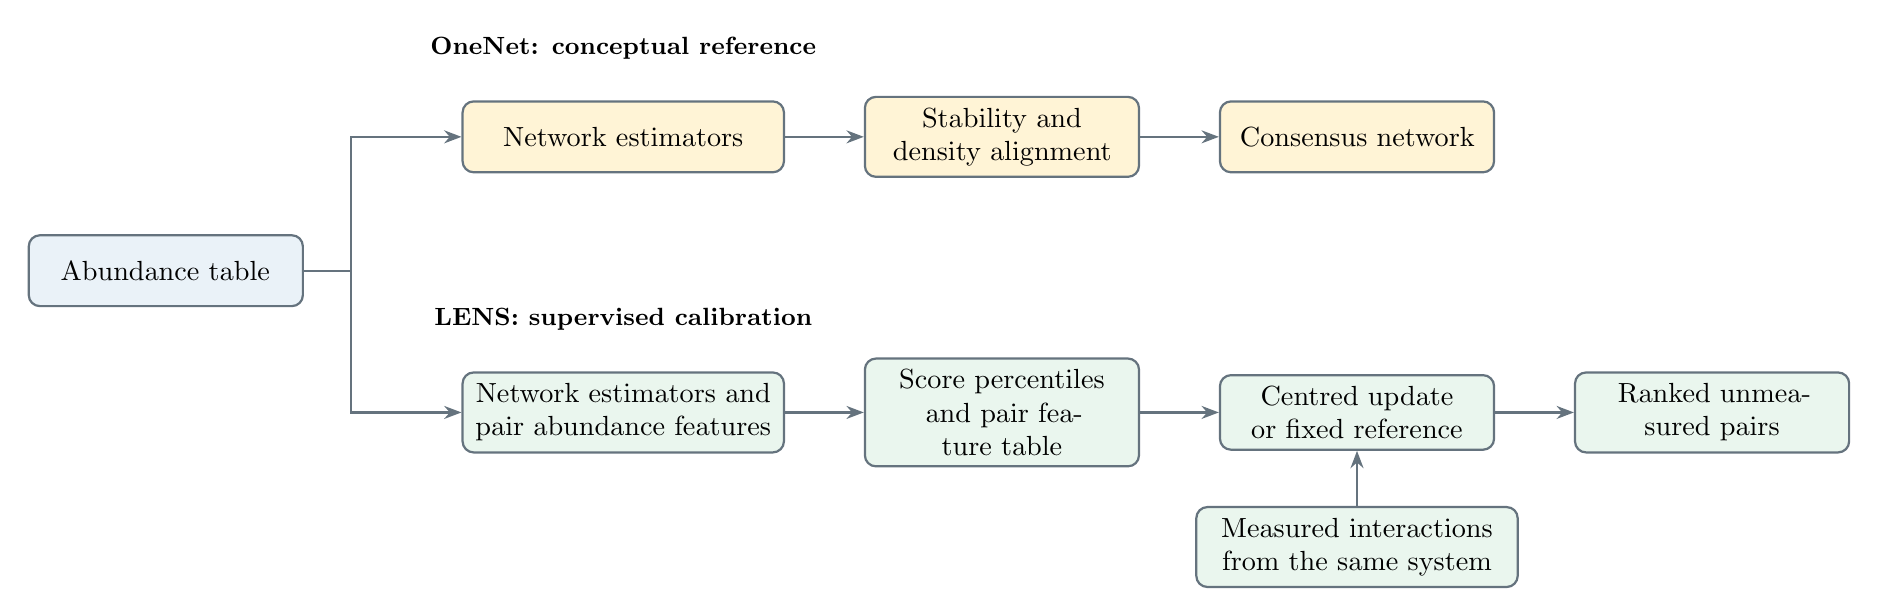
\begin{tikzpicture}[
  node distance=7mm and 10mm,
  box/.style={rounded corners, draw=linegray, thick, align=center, minimum height=9mm, text width=32mm, inner sep=4pt},
  common/.style={box, fill=bluebox},
  one/.style={box, fill=goldbox},
  sup/.style={box, fill=greenbox},
  arr/.style={-{Stealth[length=2.2mm]}, thick, draw=linegray},
  group/.style={font=\small\bfseries, align=center}
]
\node[common] (abund) {Abundance table};

\node[one, right=20mm of abund, yshift=17mm, text width=38mm] (oneestim) {Network estimators};
\node[one, right=of oneestim] (stability) {Stability and density alignment};
\node[one, right=of stability] (consensus) {Consensus network};
\node[group, above=4mm of oneestim] (onetitle) {OneNet: conceptual reference};
\draw[arr] (abund.east) -- ++(6mm,0) |- (oneestim.west);
\draw[arr] (oneestim) -- (stability);
\draw[arr] (stability) -- (consensus);

\node[sup, right=20mm of abund, yshift=-18mm, text width=38mm] (supestim) {Network estimators and pair abundance features};
\node[sup, right=of supestim] (scores) {Score percentiles and pair feature table};
\node[sup, right=of scores] (cal) {Centred update or fixed reference};
\node[sup, right=of cal] (prob) {Ranked unmeasured pairs};
\node[sup, below=of cal, text width=38mm] (labels) {Measured interactions from the same system};
\node[group, above=4mm of supestim] (suptitle) {LENS: supervised calibration};
\draw[arr] (abund.east) -- ++(6mm,0) |- (supestim.west);
\draw[arr] (supestim) -- (scores);
\draw[arr] (scores) -- (cal);
\draw[arr] (labels) -- (cal);
\draw[arr] (cal) -- (prob);

\end{tikzpicture}
}
\caption{Conceptual workflows for OneNet and LENS.}
\label{fig:workflow}
\end{figure}

\subsection{Distributed pair sampling with a fixed test set}

The primary experiment uses five held-out pair folds (\cref{fig:distributed}). Each pair identifier occurs in one test fold. Training pairs are drawn from the other four folds without using their outcomes. The samples are nested: the 40\% sample contains the pairs used at 20\%, and the same rule continues through 80\%. The unsupervised scores and test pairs stay fixed across budgets within each fold. Any change in supervised performance within a fold therefore follows from the added training labels. Figure~\ref{fig:distributed}A illustrates the 40\% budget with five schematic taxa and their 10 possible undirected pairs. Four outcomes are used for training, two are reserved for testing, and four remain unmeasured. Figure~\ref{fig:distributed}B shows how every pair enters one test fold while training pairs are drawn from the other folds.

\begin{figure}[t]
\centering
\resizebox{\textwidth}{!}{%
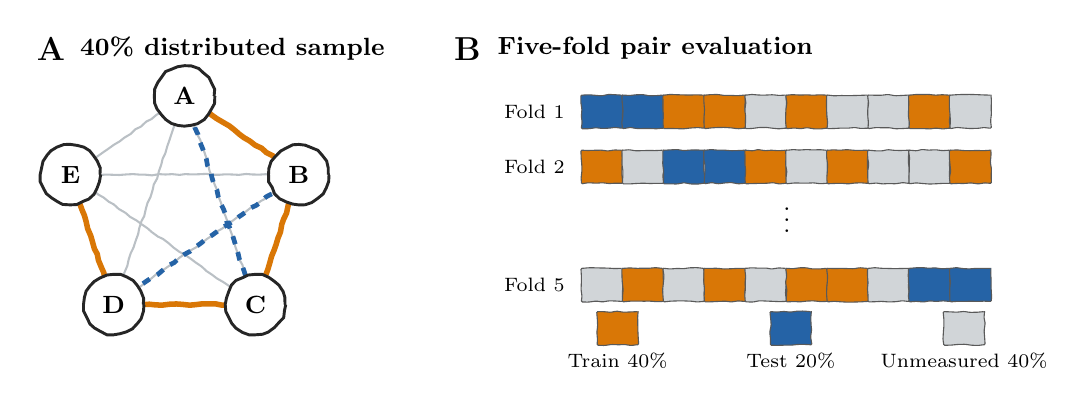
\begin{tikzpicture}[
  sketch/.style={decorate, decoration={random steps, segment length=2.4pt, amplitude=.28pt}},
  candidate/.style={draw=linegray!45, line width=0.75pt, sketch},
  measured/.style={draw=measureorange, line width=2.0pt, sketch},
  held/.style={draw=testblue, line width=1.7pt, dashed, sketch},
  taxon/.style={circle, draw=black!85, fill=white, line width=1.05pt, sketch,
    minimum size=7.5mm, inner sep=0pt, font=\small\bfseries},
  paircell/.style={rectangle, rounded corners=.35pt, draw=black!65,
    line width=.4pt, sketch, minimum width=5.2mm,
    minimum height=4.2mm, inner sep=0pt, outer sep=0pt}
]
% Panel A: one distributed-pair example.
\begin{scope}[xshift=0cm]
  \node[anchor=west, font=\large\bfseries] at (0,1.35) {A};
  \node[anchor=west, font=\small\bfseries] at (.55,1.35) {40\% distributed sample};
  % All 10 possible undirected pairs among five taxa.
  \draw[candidate]
    (2,.75)--(3.45,-.25) (2,.75)--(2.9,-1.9) (2,.75)--(1.1,-1.9)
    (2,.75)--(.55,-.25)
    (3.45,-.25)--(2.9,-1.9) (3.45,-.25)--(1.1,-1.9) (3.45,-.25)--(.55,-.25)
    (2.9,-1.9)--(1.1,-1.9) (2.9,-1.9)--(.55,-.25)
    (1.1,-1.9)--(.55,-.25);
  \draw[held]
    (2,.75)--(2.9,-1.9) (3.45,-.25)--(1.1,-1.9);
  \draw[measured]
    (2,.75)--(3.45,-.25) (3.45,-.25)--(2.9,-1.9)
    (2.9,-1.9)--(1.1,-1.9) (1.1,-1.9)--(.55,-.25);
  \node[taxon] at (2,.75) {A};
  \node[taxon] at (3.45,-.25) {B};
  \node[taxon] at (2.9,-1.9) {C};
  \node[taxon] at (1.1,-1.9) {D};
  \node[taxon] at (.55,-.25) {E};
\end{scope}

% Panel B: five-fold pair evaluation.
\begin{scope}[xshift=5.3cm]
  \node[anchor=west, font=\large\bfseries] at (0,1.35) {B};
  \node[anchor=west, font=\small\bfseries] at (.55,1.35) {Five-fold pair evaluation};

  \node[anchor=east, font=\scriptsize] at (1.65,.55) {Fold 1};
  \foreach \i/\c in {0/testblue,1/testblue,2/measureorange,3/measureorange,4/linegray!30,5/measureorange,6/linegray!30,7/linegray!30,8/measureorange,9/linegray!30}
    \node[paircell, fill=\c] at (2.0+.52*\i,.55) {};

  \node[anchor=east, font=\scriptsize] at (1.65,-.15) {Fold 2};
  \foreach \i/\c in {0/measureorange,1/linegray!30,2/testblue,3/testblue,4/measureorange,5/linegray!30,6/measureorange,7/linegray!30,8/linegray!30,9/measureorange}
    \node[paircell, fill=\c] at (2.0+.52*\i,-.15) {};

  \node[font=\small] at (4.35,-.72) {$\vdots$};

  \node[anchor=east, font=\scriptsize] at (1.65,-1.65) {Fold 5};
  \foreach \i/\c in {0/linegray!30,1/measureorange,2/linegray!30,3/measureorange,4/linegray!30,5/measureorange,6/measureorange,7/linegray!30,8/testblue,9/testblue}
    \node[paircell, fill=\c] at (2.0+.52*\i,-1.65) {};

  \node[paircell, fill=measureorange] at (2.2,-2.20) {};
  \node[font=\scriptsize] at (2.2,-2.62) {Train 40\%};
  \node[paircell, fill=testblue] at (4.4,-2.20) {};
  \node[font=\scriptsize] at (4.4,-2.62) {Test 20\%};
  \node[paircell, fill=linegray!30] at (6.6,-2.20) {};
  \node[font=\scriptsize] at (6.6,-2.62) {Unmeasured 40\%};
\end{scope}
\end{tikzpicture}
}
\caption{Distributed pair sampling and five-fold evaluation at the 40\% measurement budget.}
\label{fig:distributed}
\end{figure}

\section{Methods}

\subsection{Experimental systems and labels}

We included systems with an abundance table resolved by taxon and experimental evidence aligned to tested pairs. A positive label required support under the published rule used for that source. A neutral label required an explicit test that did not meet the rule. Untested pairs were excluded. Direction was preserved when reported.

The primary analysis used Butyrate assembly \citep{clark2021butyrate}, the Carlstr\"om removal experiment \citep{carlstrom2019}, and the Sch\"afer addition experiment \citep{schafer2022}.

\begin{table}[t]
\centering
\begin{threeparttable}
\caption{Experimental systems used in the primary analysis.}
\label{tab:systems}
\small
\begin{tabularx}{\textwidth}{@{}>{\raggedright\arraybackslash}p{0.24\textwidth}rrr>{\centering\arraybackslash}p{0.16\textwidth}>{\raggedright\arraybackslash}X@{}}
\toprule
System & Samples & Taxa & \shortstack{Tested\\pairs} & \shortstack{Class\\imbalance} & Experimental outcome \\
\midrule
Butyrate assembly \citep{clark2021butyrate} & 537 & 26 & 104 & 2.71 & Effects derived from synthetic gut assembly \\
Carlstr\"om \citep{carlstrom2019} & 48 & 55 & 989 & 7.04 & Removal effects in an Arabidopsis consortium \\
Sch\"afer \citep{schafer2022} & 662 & 127 & 1,524 & 39.11 & Addition effects in an Arabidopsis consortium \\
\bottomrule
\end{tabularx}
\begin{tablenotes}[flushleft]\footnotesize
\item Taxa are those represented among tested pairs. Class imbalance is the number in the majority class divided by the number in the minority class. Positive outcomes form the majority in Butyrate; neutral outcomes form the majority in Carlstr\"om and Sch\"afer.
\end{tablenotes}
\end{threeparttable}
\end{table}

\subsection{Abundance preparation and pair features}

Abundance matrices were aligned to the taxa in each truth table. Methods that required values similar to counts received a documented conversion when the source matrix was noninteger and nonnegative: each sample was rescaled to a total of 10,000 and rounded. This supplies a compatible numerical input and does not recover original sequence counts. Presence was defined as an abundance greater than zero.

The calibrated model used score percentiles from PLNNetwork, Poisson GLMNet, and SparCC. Eleven abundance features described prevalence, joint detection, similarity of presence patterns, association among all samples and among jointly observed samples, log ratio variance, and abundance contrasts. All features were computed without interaction outcomes.

\subsection{Unsupervised estimators}

PLNNetwork used a Poisson lognormal model and sparse precision estimation as implemented in PLNmodels 1.2.2 \citep{chiquet2019pln}. Poisson neighborhood selection fitted one penalized Poisson regression per taxon using glmnet 4.1-8 \citep{allen2013poisson,friedman2010glmnet}. SPIEC-EASI 1.99.0 used centered log ratio preprocessing, graphical lasso, 50 penalty values, a minimum to maximum penalty ratio of 0.05, and StARS selection \citep{kurtz2015spieceasi}. SparCC supplied marginal compositional association scores \citep{friedman2012sparcc}. The mean rank was the mean of the PLNNetwork, Poisson GLMNet, and SparCC score percentiles.

The OneNet sensitivity run used OneNet 0.3.1 with PLNnetwork, SPIEC-EASI, gCoda, EMtree, Magma, and SPRING \citep{champion2024onenet}. Thirty resamples were used. Penalty paths were aligned at mean stability 0.8, following the package tutorial, and the consensus score was the mean edge selection frequency. ZiLN was excluded after it failed on resamples containing constant taxon columns. We retained the full taxon set so that OneNet and the other methods were scored on the same test pairs.

Experimental outcomes did not enter network fitting, tuning, or score construction. The primary score for each method was the percentile of absolute edge strength within the abundance table. The full comparison evaluated every method separately. The oracle summary selected the method with the largest mean AUPRC for each system after all test results had been calculated.

\subsection{LENS calibration model}

LENS treated a supported interaction as one and a tested neutral as zero. The fixed reference score, the centred update, and the evidence rule below define the prediction procedure. For pair $i$, the centred branch estimated
\begin{equation}
p_i = \Pr(Y_i=1\mid\mathbf{x}_i)
    = \operatorname{logit}^{-1}\!\left(\alpha+\mathbf{x}_i^{\mathsf T}\boldsymbol\beta\right),
\label{eq:calibration-probability}
\end{equation}
where $\mathbf{x}_i$ contains the three network score percentiles and 11 abundance features. The intercept $\alpha$ was unpenalized.

We fitted the coefficients with balanced class weights and a ridge penalty centred on a reference vector:
\begin{equation}
(\widehat\alpha,\widehat{\boldsymbol\beta})
= \arg\min_{\alpha,\boldsymbol\beta}
\left[
-\sum_{i\in\mathcal{T}} w_i
\left\{Y_i\log p_i+(1-Y_i)\log(1-p_i)\right\}
+\frac{\lambda}{2}\left\|\boldsymbol\beta-\boldsymbol\beta_{0}\right\|_2^2
\right].
\label{eq:centered-ridge}
\end{equation}
Here, $\mathcal{T}$ is the set of measured training pairs and $w_i$ balances the two outcome classes. On the original percentile scale, the reference vector was
\begin{equation}
\boldsymbol\beta_{0}
= \left(\tfrac{1}{3},\tfrac{1}{3},\tfrac{1}{3},0,\ldots,0\right)^{\mathsf T}.
\label{eq:ridge-center}
\end{equation}
The first three entries correspond to PLNNetwork, Poisson GLMNet, and SparCC. The remaining entries correspond to abundance features. Strong regularization returns the model toward the equal mean of the three network scores. Measured interactions can support different weights and contributions from the abundance features. The reference is therefore part of the fitted model, not a separate comparator.

Candidate penalty values were $\lambda=0.01$, $0.1$, $1$, and $10$. Three-fold stratified inner validation selected $\lambda$ by mean AUPRC. Missing predictors were imputed with the training median, and predictors were standardized using the training sample. The reference coefficients were adjusted after standardization so that they retained the ranking defined in \cref{eq:ridge-center}. The random seed was 20260821.

When either outcome class contained fewer than three measured pairs, stratified inner validation was unavailable. The procedure then remained at its reference ranking and used
\begin{equation}
s_i^{\mathrm{fixed}}=\frac{s_{i,\mathrm{PLN}}+s_{i,\mathrm{GLMNet}}+s_{i,\mathrm{SparCC}}}{3}.
\label{eq:fixed-score}
\end{equation}
The class count therefore determines whether LENS retains its reference or estimates an update. The fallback uses no experimental outcome beyond that decision. No outer test outcome entered imputation, scaling, fitting, penalty selection, or training pair selection.

\subsection{Exploratory analysis of effect sign}

Carlstr\"om was the only system with enough positive and negative effects for a separate sign analysis. Taxon names within each pair were placed in a fixed order before the truth and feature tables were joined. This recovered 86 pairs that appeared in opposite orders across the two files. Another 160 pairs involved five taxa absent from the abundance table and were excluded. The scored set contained 989 pairs: 105 positive effects, 18 negative effects, and 866 tested neutral outcomes.

We fitted a multinomial ridge model with class weights to the signed PLNNetwork, Poisson GLMNet, and SparCC scores; their absolute score percentiles; and four prevalence features. Five outer folds produced one held-out prediction for every pair. Three inner stratified folds selected $C$ from 0.001, 0.01, 0.1, 1, and 10 by macro average precision. For the network display, each training fold supplied its observed interaction frequency. That frequency fixed the number of edges selected from its test fold. LENS ranked pairs by one minus the predicted neutral probability, and OneNet ranked the same pairs by its consensus score. Experimental outcomes were used to color the selected edges after prediction.

\subsection{Five-fold evaluation and nested budgets}

For distributed sampling, five outer folds partitioned the tested pair identifiers. Fold construction used the pair outcome to balance the positive frequency where the number of positive and neutral pairs permitted it. Each pair identifier occurred in one test fold. This fixed test construction separates evaluation pairs from the interaction measurements available to LENS. Training pair identifiers were placed in a random order without using outcomes. Nested samples contained 20\%, 40\%, 60\%, or 80\% of all tested pair identifiers, capped by the four-fold training pool. At 80\%, every pair outside the test fold was used for training.

The test pair identifiers stayed fixed across budgets within an outer fold. Unsupervised methods were fitted once to the full abundance table. LENS was applied again at each budget, starting from the same reference score. Three inner pair folds selected the penalty when both outcome classes contained at least three measured pairs. Smaller samples remained on the fixed mean score. The budget comparison therefore follows one procedure from its unsupervised reference through increasingly informed supervised updates.

For the taxon panel sensitivity analysis, 40\% of taxa were reserved for testing in each repeat. Test pairs contained two reserved taxa. The training pool contained pairs formed only from the remaining taxa. Budgets contained 20\%, 40\%, 60\%, or 80\% of eligible pair identifiers and were nested. The taxon partition and test pairs stayed fixed across budgets. This analysis used L2 logistic regression with $C=0.01$ and balanced class weights; it is reported separately from the primary centred ridge analysis.

\subsection{Evaluation}

The primary metric was average precision, reported as AUPRC. The prediction task was to rank experimentally supported interactions above tested neutral pairs, and the outcome frequencies were strongly imbalanced in Carlstr\"om and Sch\"afer. In Sch\"afer, only 38 of 1,524 tested pairs were positive. A classifier that labeled every pair neutral would therefore achieve 97.5\% accuracy while recovering no supported interaction. Accuracy would reward the dominant class without measuring the purpose of the model.

AUPRC summarizes precision across the recall values induced by the complete ranking and gives greater attention to recovery of the positive class \citep{saito2015}. Its uninformative baseline equals the positive frequency, which was reported for each system. This baseline makes clear how much a ranking improves on the class distribution. AUROC was secondary because the large number of neutral pairs can produce a favorable false positive rate even when many neutral pairs appear above the rare positives. Precision, recall, and F1 require a selected threshold or edge count, so they were used for specific graph comparisons and were not the primary measure of the full ranking.

We report means and standard deviations across the five outer test folds. The folds share one biological system, so their standard deviation describes variation among held-out pair sets and does not measure variation across independent systems.

\section{Results}

The analysis used Butyrate assembly, Carlstr\"om, and Sch\"afer (\cref{tab:systems}). Each source supplied an abundance table and explicit undirected outcomes for tested pairs. Untested pairs were excluded. Butyrate contained substantially more positive outcomes than the two plant systems. Sch\"afer had the strongest class imbalance, with 38 positive and 1,486 neutral outcomes.

\subsection{Unsupervised estimators differed across systems}

The unsupervised methods were fitted once per abundance table and did not use interaction outcomes. Their scores were constant across measurement budgets. The supervised comparison used OneNet as a prespecified reference in every system. This avoids choosing an unsupervised estimator after inspecting experimental outcomes.

The method with the largest mean AUPRC changed across the three experimental systems (\cref{fig:unsupervised-full-auprc}). The bars show the mean across five abundance resamples for PLNNetwork, Poisson GLMNet, SparCC, and SPIEC-EASI. Capped error bars show one standard deviation across those refits. OneNet already performs internal resampling, so its bar shows the fit to the complete abundance table without an external error bar. The red dotted line gives the positive interaction frequency, which is the expected AUPRC of an uninformative ranking. The systems contained 104, 989, and 1,524 tested pairs, and the horizontal scales differ so that performance within each system remains visible.

\begin{figure}[!t]
\centering
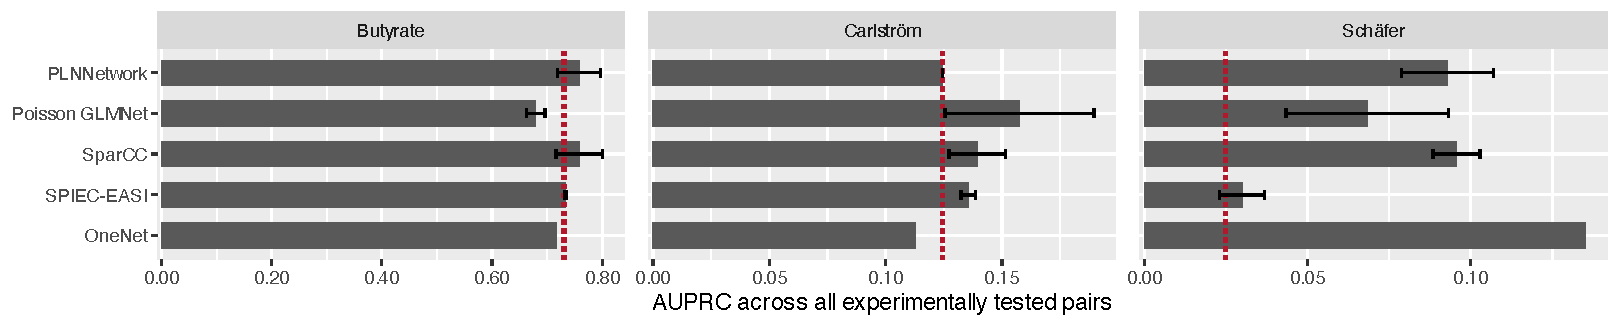
\includegraphics[width=\textwidth]{figures/unsupervised_full_tested_pair_auprc.pdf}
\caption{AUPRC of unsupervised network estimators across experimentally tested pairs.}
\label{fig:unsupervised-full-auprc}
\end{figure}

\subsection{LENS improved ranking at the 80\% budget}

At the 80\% measurement budget, LENS exceeded OneNet by 0.166 AUPRC in Butyrate, 0.157 in Carlstr\"om, and 0.248 in Sch\"afer. Table~\ref{tab:lens-onenet-discrimination} reports AUPRC and AUROC for LENS, OneNet, SparCC, and SPIEC-EASI from the same five held-out pair folds. Figure~\ref{fig:final-pr-curves} also includes PLNNetwork, one of the three scores used by LENS. SparCC and SPIEC-EASI represent marginal association and sparse conditional dependence. The ribbons give one standard error around mean precision. Every prediction came from the fold in which that pair was held out. Positive interaction frequencies were 0.731 in Butyrate, 0.124 in Carlstr\"om, and 0.025 in Sch\"afer, which explains the different precision ranges.

\begin{table}[!t]
\centering
\caption{Discrimination at the 80\% interaction measurement budget.}
\label{tab:lens-onenet-discrimination}
\small
\setlength{\tabcolsep}{3.8pt}
\begin{tabular}{lcccccccc}
\toprule
System & \multicolumn{4}{c}{AUPRC} & \multicolumn{4}{c}{AUROC} \\
\cmidrule(lr){2-5}\cmidrule(lr){6-9}
& LENS & OneNet & SparCC & SPIEC-EASI & LENS & OneNet & SparCC & SPIEC-EASI \\
\midrule
Butyrate & \textbf{0.882} & 0.717 & 0.806 & 0.734 & \textbf{0.755} & 0.408 & 0.566 & 0.507 \\
Carlstr\"om & \textbf{0.282} & 0.125 & 0.125 & 0.140 & \textbf{0.705} & 0.468 & 0.453 & 0.504 \\
Sch\"afer & \textbf{0.429} & 0.181 & 0.147 & 0.025 & \textbf{0.941} & 0.846 & 0.891 & 0.499 \\
\bottomrule
\end{tabular}
\end{table}

\begin{figure}[!t]
\centering
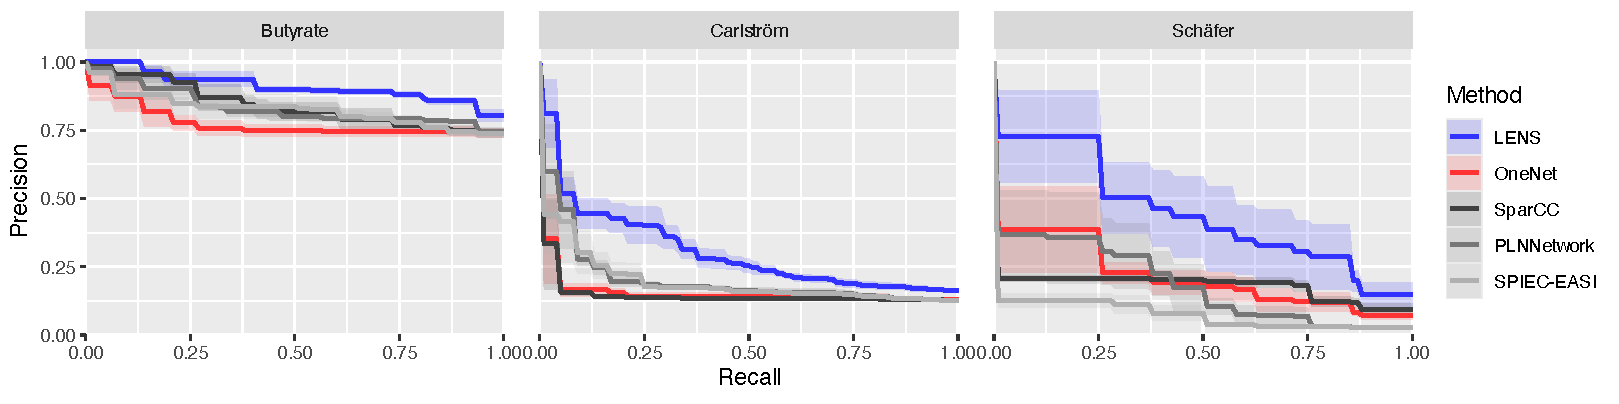
\includegraphics[width=\textwidth]{figures/final_sparse_pr_curves.pdf}
\caption{Precision--recall curves for LENS and four unsupervised comparators at the 80\% measurement budget.}
\label{fig:final-pr-curves}
\end{figure}

\clearpage
\subsection{AUPRC increased with the measurement budget}

\begin{figure}[!t]
\centering
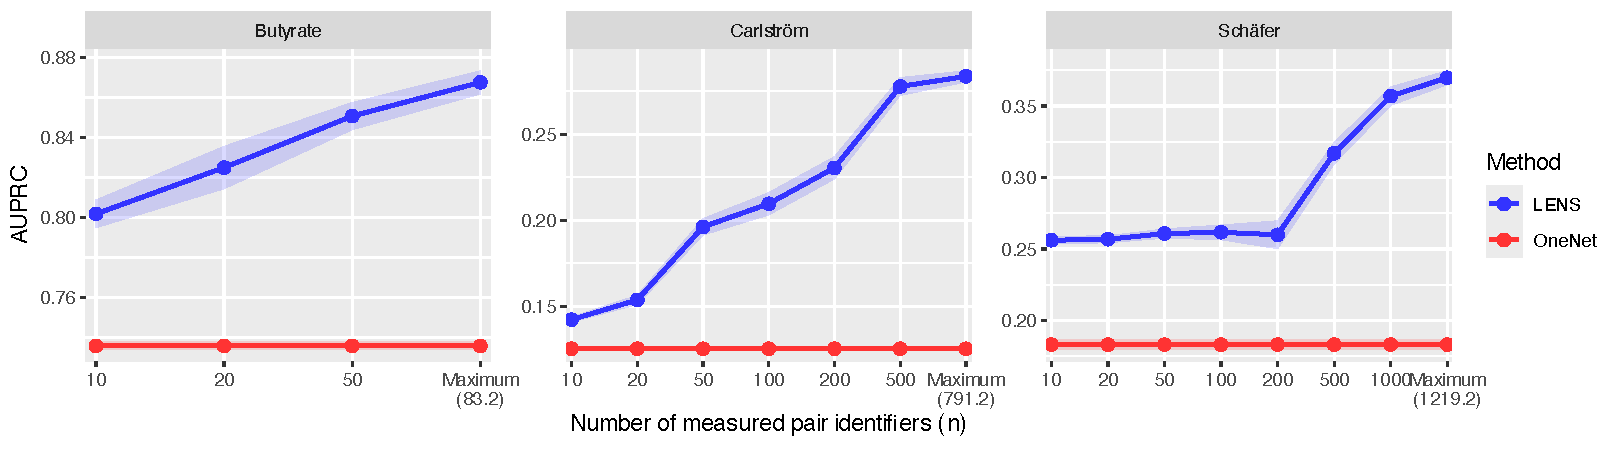
\includegraphics[width=\textwidth]{figures/butyrate_absolute_pair_budgets.pdf}
\caption{AUPRC across absolute interaction measurement budgets.}
\label{fig:absolute-pair-budget}
\end{figure}

Figure~\ref{fig:absolute-pair-budget} reports 20 repeated five-fold partitions at fixed numbers of measured pairs. Lines show mean AUPRC and ribbons give one standard error across the repeated partitions. Pair samples were nested and selected without their outcomes. The maximum used every pair outside the held-out fold, giving mean training counts of 83.2 in Butyrate, 791.2 in Carlstr\"om, and 1,219.2 in Sch\"afer. OneNet was scored on the same test pairs and remained independent of the interaction outcomes. Separate vertical scales preserve the changes within each system.

LENS exceeded OneNet at every absolute budget in all three systems. Mean AUPRC increased from 0.802 to 0.868 in Butyrate and from 0.142 to 0.284 in Carlstr\"om. Sch\"afer remained near 0.26 through 200 measured pairs, then increased to 0.317 at 500 pairs and 0.370 at the maximum. The fixed mean score protected the ranking when too few interactions from either class were available for inner validation. Once both classes had at least three measured pairs, stratified inner validation selected the ridge penalty. This design lets LENS remain close to the unsupervised evidence when labels are weak and learn a new combination when the measured interactions are informative.

\subsection{LENS recovered more signed experimental edges in Carlstr\"om}

Figure~\ref{fig:carlstrom-signed-network} compares the 123 experimentally supported effects with equal edge selections from LENS and OneNet. Both methods selected 125 held-out pairs using the edge count derived from training data. LENS recovered 28 positive and four negative effects, giving a precision of 0.256 and recall of 0.260. OneNet recovered nine positive and two negative effects, giving a precision of 0.088 and recall of 0.089. Grey edges in the prediction panels are selected pairs that were experimentally neutral.

The signed model improved average precision for positive effects from 0.114 for the strongest individual score to 0.189. Average precision for negative effects was 0.017, close to the negative frequency of 0.018. The figure shows recovery of experimentally supported interactions with known signs. It does not show reliable prediction of the effect sign itself.

\begin{figure}[!t]
\centering
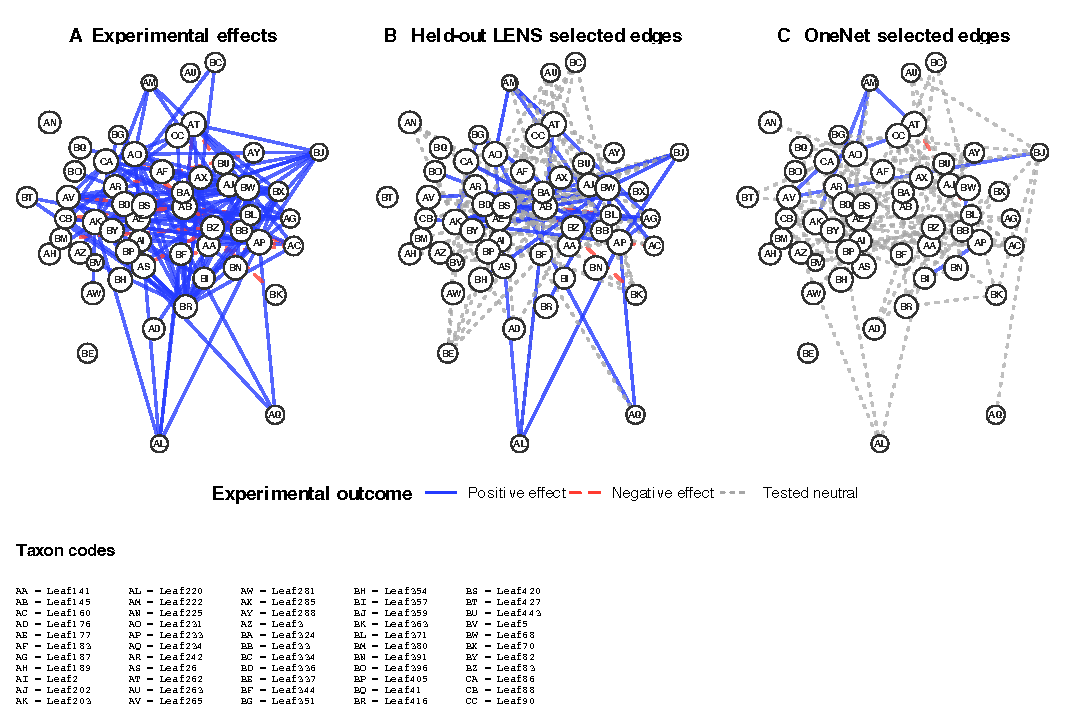
\includegraphics[width=\textwidth]{figures/carlstrom_signed_network.pdf}
\caption{Experimental effects and equal edge selections from LENS and OneNet in Carlstr\"om.}
\label{fig:carlstrom-signed-network}
\end{figure}

\FloatBarrier
\section{Discussion}

The central result concerns measurement allocation within a single prediction procedure. LENS begins with a fixed abundance-derived ranking, retains that ranking when the measured pairs contain insufficient class evidence, and estimates a centred update once both classes support validation. Every budget used the same test pairs within an outer fold, so changes in test composition cannot explain the increase. The gain was gradual in Butyrate and Carlstr\"om. In Sch\"afer, little changed through 200 measured pairs before the ranking improved at 500 pairs. The number of useful measurements therefore depends on the frequency of supported effects and on how much information the abundance scores contain for the experimental endpoint.

This result gives each component of LENS a specific role. The equal mean supplies a prespecified ranking before adequate labels exist. The centred penalty limits how far a small interaction screen can move that ranking. Pair abundance features enter through the same update, and the fixed test construction isolates the effect of adding labels. Researchers can retain the broad coverage of an abundance experiment and add a smaller interaction screen where laboratory capacity permits. Related supervised approaches use traits or previous interaction measurements to predict unperformed experiments \citep{dimucci2018missing,nestor2023growth}. LENS addresses the setting in which abundance measurements already exist and the interaction screen can cover only part of the same taxon set.

Where the measurements are placed also matters. The taxon panel sensitivity analysis reserved 40\% of taxa in each repeat and used the original fixed L2 logistic specification. Training labels came only from pairs among the remaining taxa, while test pairs were formed among reserved taxa. The unsupervised scores still used the complete abundance table. At the 80\% budget, calibration exceeded the oracle reference in Carlstr\"om, was close to SparCC in Butyrate, and remained below mean rank in Sch\"afer. Sch\"afer improved from 0.150 at 20\% to 0.245 at 80\%, compared with 0.301 for mean rank. These results indicate that measurements spread across the taxa gave more consistent gains than labels confined to one panel.

A laboratory with a fixed measurement capacity may therefore gain more from sampling pairs across many taxa than from completing a dense block for a few taxa. Work on active learning for biological networks formalizes the next step: choose experiments by expected information or cost, then update the model with the observed outcomes \citep{sverchkov2017active}. Our experiment used random distributed sampling, so it does not identify the best pairs to measure. It provides the reference against which an adaptive rule should be tested.

The unsupervised comparison helps explain why calibration can help. The leading estimator changed across systems, and no single score dominated the three benchmarks. This agrees with earlier comparisons in which tool choice changed edge recovery and network properties \citep{weiss2016correlation,rottjers2018hairballs}. OneNet gives a prespecified consensus without interaction outcomes \citep{champion2024onenet}. LENS uses partial outcomes to change the contribution of the scores and abundance features. In Carlstr\"om, it recovered 32 supported effects at the selected edge count, compared with 11 for OneNet. This comparison used identical test pairs and an equal number of selected edges.

The sign analysis was less successful. LENS ranked positive effects better than the individual signed scores, but average precision for negative effects remained near their frequency. Only 18 negative effects were available, and the network scores were symmetric even though experimental effects can be directional. The Carlstr\"om network should therefore be read as an interaction recovery example with experimentally known signs. It does not establish sign prediction.

\section{Limitations}

The study contains three microbial systems. Their experiments measured different biological responses: assembly, removal, and addition effects. A statistical association can agree with one response and disagree with another without either analysis being erroneous. The present results establish performance for these three sources; they do not estimate an average effect across microbial experiments.

The validation folds reserve pairs within a system. Pairs in the same source share taxa, abundance samples, laboratory procedures, and outcome definitions. Five-fold validation prevents direct reuse of a pair label, but it does not create five independent biological experiments. Standard errors and variation among folds describe sensitivity to the pair partition. They should not be interpreted as uncertainty across new microbial systems.

Experimental labels also require care. Untested pairs were excluded, and tested neutral pairs were kept separate from missing outcomes. The primary analysis combined positive and negative experimental effects into one interaction class. This was appropriate for unsigned recovery, but it removed direction and sign from the main target. The signed analysis restored effect sign only for Carlstr\"om and remained limited by 18 negative examples. Some experimental pairs could not be scored because their taxa were absent from the aligned abundance table.

The abundance sources used different measurement scales. Two systems supplied integer amplicon counts, while Butyrate supplied proportions that were converted to count-like values for methods requiring nonnegative integers. That conversion provides compatible input and cannot reconstruct original sequencing counts. Method failures and software availability also limited the estimator set. OneNet used its internal resampling on the complete abundance table; we did not add external abundance resampling to the budget analysis.

AUPRC was the primary metric because supported effects were rare in two systems. Its baseline equals the positive frequency, so raw values cannot be compared across systems without the class balance. The network display used an edge count derived from the training interaction frequency. This makes LENS and OneNet comparable at one density, though a prospective study would need to choose its reporting threshold before revealing the unmeasured outcomes.

\section{Future work}

The next test should be prospective. Researchers could select an initial distributed sample of pairs, fit LENS, and then perform a second set of experiments chosen from the unmeasured pairs. This would test whether the ranking saves experiments when the outcomes are unavailable at the time of selection. It would also permit a direct accounting of laboratory time and cost.

Pair selection can also be improved. Random sampling provides a clear reference, but it may spend measurements on pairs that add similar information. Active learning studies of biological networks have used entropy, disagreement between competing models, and expected experimental cost to select new measurements \citep{sverchkov2017active}. A LENS extension could favor taxa with little experimental coverage, pairs for which the estimators disagree, or predictions with high uncertainty. Any such rule must be fixed using training data and evaluated on a reserved set. Comparison with random distributed sampling would show whether adaptation adds value beyond a larger budget.

More experimental systems are needed before fitting study effects or a shared calibration rule. With enough sources, a hierarchical model could borrow information across assays while allowing the score weights to differ. Repeated experiments using similar taxa under different media or hosts would be especially useful because they would separate transfer across organisms from transfer across experimental conditions.

Sign and direction require different predictors. Genome traits, metabolic features, monoculture growth, and ordered source and target features may help distinguish facilitation from inhibition. A directional extension should preserve $A\rightarrow B$ and $B\rightarrow A$ as separate outcomes and keep reciprocal directions in the same validation fold. Probability calibration, stopping rules for measurement, and precision at a laboratory edge budget should accompany discrimination metrics in that work.

\section{Conclusion}

Partial interaction measurements improved the ranking of unmeasured pairs in three microbial systems when they were distributed across the available taxa. LENS links a prespecified network score, a centred supervised update, and an evidence-based fallback in one procedure that remains defined across measurement budgets. Fixed test pairs showed how the same ranking changed as interaction outcomes entered training. The result supports a study design in which abundance data guide a partial interaction screen and the measured outcomes guide the remaining experiments. Evidence for sign prediction is still inadequate, and confirmation in independent prospective systems is needed.

\section{Software and reproducibility}

Analyses were run in R and Python with recorded package versions and fixed random seeds. Cached estimator fits, pair features, repeat results, summary tables, exclusions, and provenance records are stored separately. Taxon pair ordering was deterministic.

\section*{Data and code availability}

The analysis repository contains the scripts, processed pair features, provenance records, and result tables needed to reproduce the analysis. Source data remain under their original licenses and are identified by article or repository DOI. A permanent public repository address and final author metadata should be added before public submission.

\section*{Acknowledgments}

The authors thank the investigators who released the abundance and interaction data used in this study.

\bibliographystyle{plainnat}
\bibliography{references}

\end{document}
